\medskip

L'espace est muni d'un repère orthonormé \Oijk{}.

On considère les points A$(5~;~5~;~0)$, B$(0~;~5~;~0)$, C$(0~;~0~;~10)$ et D$\left(0~;~0 ~;~-\dfrac{5}{2}\right)$.

\begin{center}
	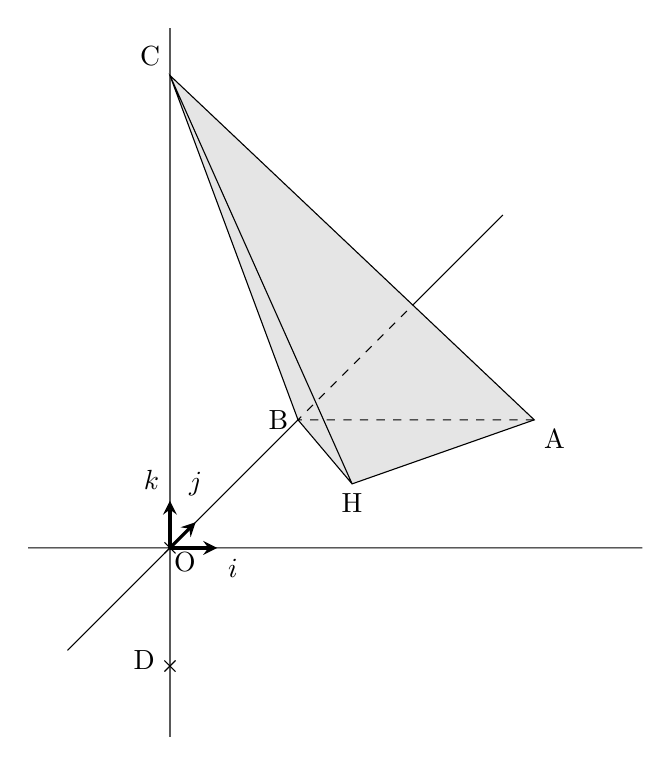
\begin{tikzpicture}[x={(0:6mm)},y={(45:4.6mm)},z={(90:6mm)},>=stealth]
		\fill[gray!20] (5,5,0)--(2.5,2.5,0)--(0,5,0)--(0,0,10)--cycle;
		\draw (5,5,0)node [below right]{A}--
		(0,0,10) node[above left]{C}--
		(0,5,0) node [left]{B}--
		(2.5,2.5,0) node [below] {H}-- cycle (0,0,10)--(2.5,2.5,0);
		\draw[line width = 1.2pt,->] (0,0,0)--(1,0,0) node [below right]{$ \vect{i} $};
		\draw[line width = 1.2pt,->] (0,0,0)--(0,1,0) node [above =2mm]{$ \vect{j} $};
		\draw[line width = 1.2pt,->] (0,0,0)--(0,0,1) node [above left]{$ \vect{k} $};
		\draw (-3,0,0)--(10,0,0) (0,0,-4)--(0,0,11) (0,-4,0)--(0,5,0) (0,9.5,0)--(0,13,0);
		\draw[shift={(0,0,-2.5)}] (-2pt,-2pt)--(2pt,2pt) (2pt,-2pt)--(-2pt,2pt) node [left]{D};
		\draw[shift={(0,0,0)}] (-2pt,-2pt)--(2pt,2pt) (2pt,-2pt)--(-2pt,2pt) node [below right]{O};
		\draw[dashed] (5,5,0)--(0,5,0)--(0,9.5,0);
	\end{tikzpicture}
\end{center}

\begin{enumerate}
	\item \begin{enumerate}
		\item Montrer que $\vect{n_{1}}\begin{pmatrix}1 \\ -1 \\ 0\end{pmatrix}$ est un vecteur normal au plan (CAD).

		\item En déduire que le plan (CAD) a pour équation cartésienne : \quad $x-y=0$.
	\end{enumerate}

	\item On considère la droite $\mathcal{D}$ de représentation paramétrique \renewcommand\arraystretch{1.8}$\left\{\begin{array}{l c l}x&=&\phantom{5 -}\dfrac{5}{2} t \\ y&=&5-\dfrac{5}{2} t \\ z&=&0\end{array}\right.$ où $t \in \R$.\renewcommand\arraystretch{1}


	\begin{enumerate}
		\item On admet que la droite $\mathcal{D}$ et le plan (CAD) sont sécants en un point H. Justifier que les coordonnées de H sont $\left(\dfrac{5}{2}~;~\dfrac{5}{2}~;~0\right)$.

		\item Démontrer que le point H est le projeté orthogonal de B sur le plan (CAD).
	\end{enumerate}

	\item \begin{enumerate}
		\item Démontrer que le triangle ABH est rectangle en H.

		\item En déduire que l'aire du triangle ABH est égale à $\dfrac{25}{4}$.
	\end{enumerate}

	\item \begin{enumerate}
		\item Démontrer que (CO) est la hauteur du tétraèdre ABCH issue de C.

		\item En déduire le volume du tétraèdre ABCH.

		\emph{On rappelle que le volume d'un tétraèdre est donné par : $V=\dfrac{1}{3} \mathcal{B }h$, où $\mathcal{B}$ est l'aire d'une base et $h$ la hauteur relative à cette base.}
	\end{enumerate}

	\item On admet que le triangle ABC est rectangle en B. Déduire des questions précédentes la distance du point H au plan (ABC).
\end{enumerate}

\medskip
